\ifx\fulldocument\undefined
\documentclass[aspectratio=169]{beamer}
% \usetheme{sdr}
\graphicspath{{./tex/imgs/}}

\usepackage[utf8]{inputenc}

\title{Programmiamo Umanoidi!}
\subtitle{}
\author{Lorenzo Leonardini}
\institute{Scuola di Robotica}
\date{\today}

\begin{document}
\fi

\begin{frame}
	\titlepage
\end{frame}

\begin{frame}
\frametitle{Indice}
\tableofcontents
\end{frame}

\section{Che cos'è NAO}

\begin{frame}
\frametitle{Che cos'è NAO}
\begin{columns}
	\column{0.5\textwidth}
		\begin{itemize}
			\item<1-> È il robot umanoide più usato al mondo in ambito educativo e medico
			\item<2-> Sviluppato a partire dal 2004 da Aldebaran Robotics
			\item<3-> Acquistata nel 2015 da SoftBank Robotics, che nel 2017 ha acquistato anche Boston Dynamics
		\end{itemize}
	\column{0.5\textwidth}
		\begin{figure}[ht]
		\begin{center}
		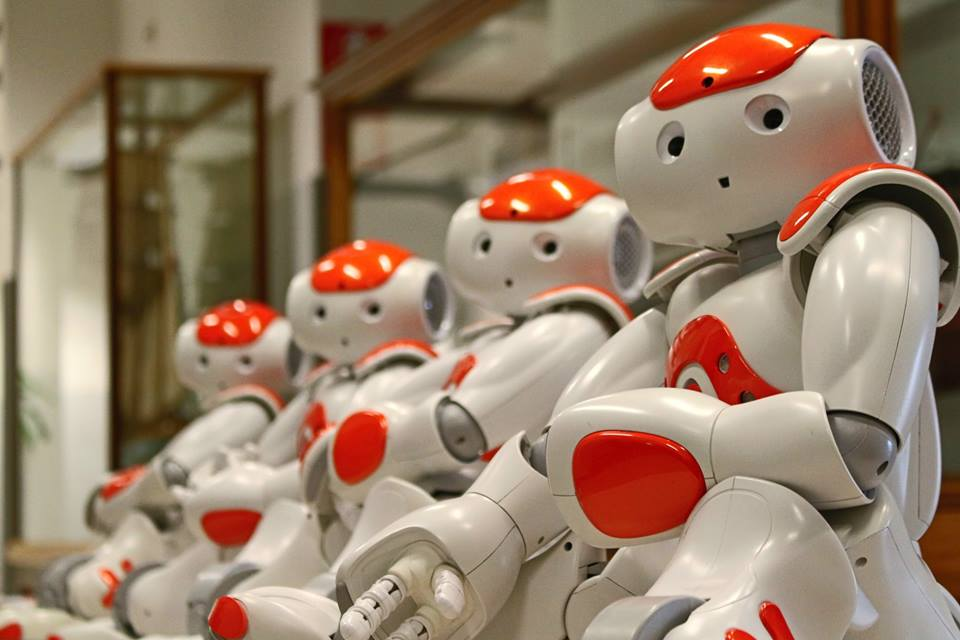
\includegraphics[width=0.9\textwidth]{nao1.jpg}<1->
		\end{center}
		\end{figure}
\end{columns}
\end{frame}

\subsection{Caratteristiche}

\begin{frame}
\frametitle{Che cos'è NAO - Caratteristiche}
\begin{columns}
	\column{0.5\textwidth}
		\begin{figure}[ht]
		\begin{center}
		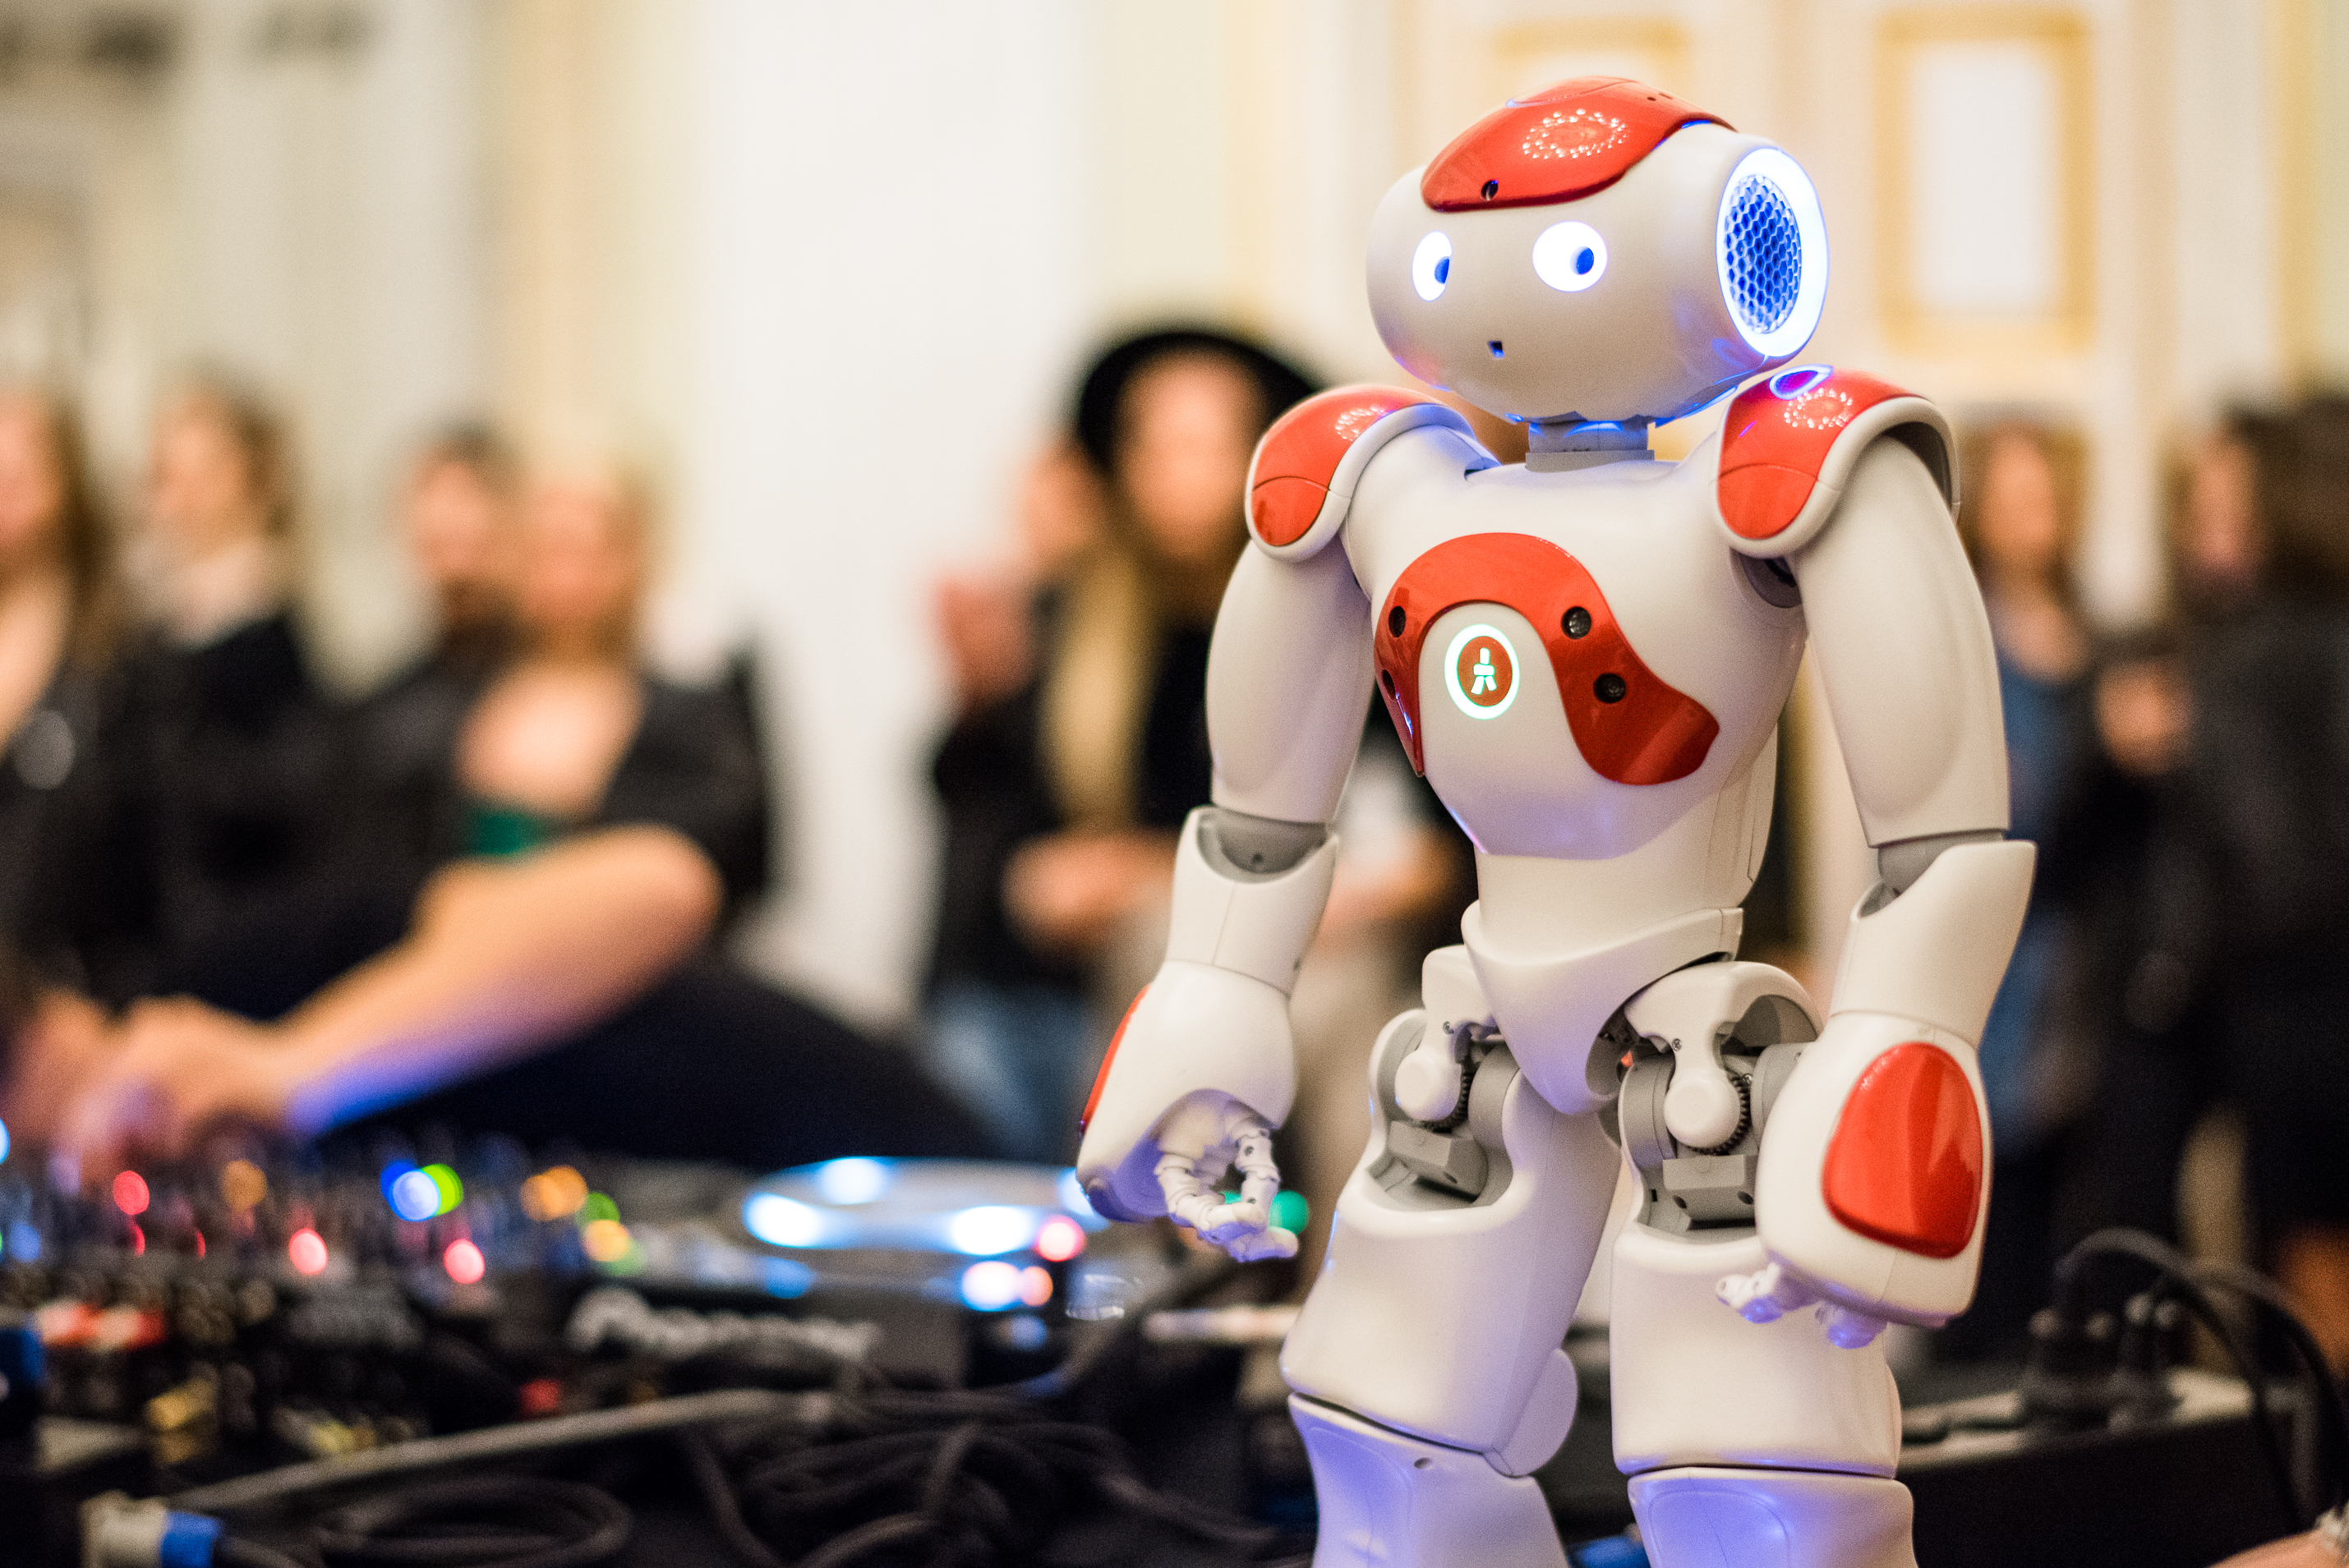
\includegraphics[width=0.9\textwidth]{nao8.jpg}<1->
		\end{center}
		\end{figure}
	\column{0.5\textwidth}
		Pensato per l'interazione con l'essere umano, sensoristica sviluppata di conseguenza:
		\begin{itemize}
			\item<2-> Sensori di tatto
			\item<3-> Riconoscimento e sintesi vocale
			\item<4-> Numerosi microfoni per localizzare la sorgente sonora
			\item<5-> Riconoscimento facciale e di oggetti
		\end{itemize}
\end{columns}
\end{frame}

\begin{frame}
\frametitle{Che cos'è NAO - Caratteristiche}
Elementi "umani" volti a mettere a proprio agio l'interlocutore:
\begin{itemize}
	\item<2-> Sembianze di un bambino e non di un adulto
	\item<3-> Sembianze "cartoonesche"
	\item<4-> Autonomous move
	\item<5-> Si guarda attorno sbattendo le palpebre
\end{itemize}
\end{frame}

\subsection{Movimento}
\begin{frame}
\frametitle{Che cos'è NAO - Movimento}
\begin{columns}
	\column{0.5\textwidth}
		\begin{itemize}
			\item<1-> 25 gradi di movimento in tutto il corpo
			\item<2-> Sensori in ogni motore per rilevare la loro posizione
			\item<3-> IMU (Intertial Measurement Unit)
			\item<4-> Bumper sui piedi
			\item<5-> Telecamera puntata per terra
			\item<6-> Coppia di ultrasuoni sul petto\\

			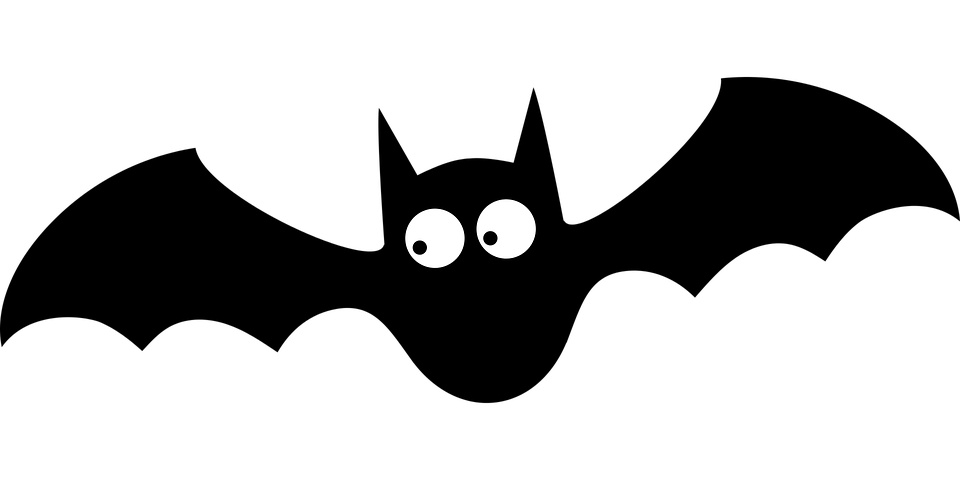
\includegraphics[width=0.3\textwidth]{pipistrello.png}<7->
		\end{itemize}
	\column{0.5\textwidth}
		\begin{figure}[ht]
		\begin{center}
		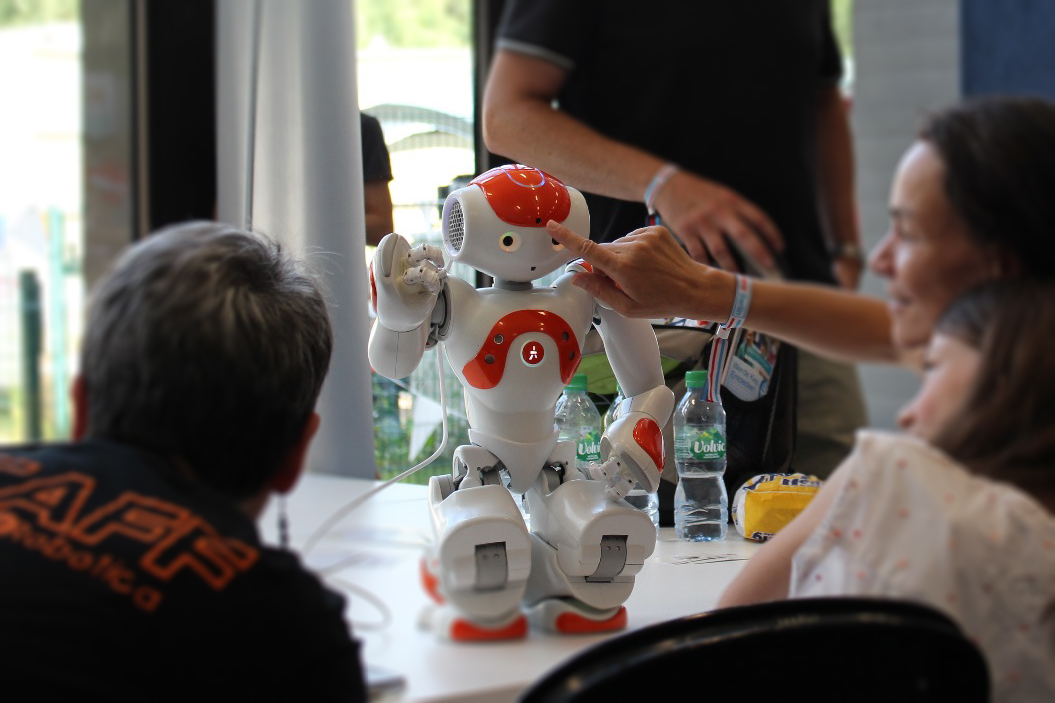
\includegraphics[width=0.9\textwidth]{nao3.jpg}<1->
		\end{center}
		\end{figure}
\end{columns}
\end{frame}

\subsection{Utilizzi}

\begin{frame}
\frametitle{Che cos'è NAO - Utilizzi}
Educazione
\begin{itemize}
	\item<2-> Introduzione alla robotica, alla programmazione
	\item<3-> Avvicinamento dei giovani alla tecnologia
\end{itemize}
Salute
\begin{itemize}
	\item<4-> Supporto agli anziani
	\item<5-> Supporto a persone con difficoltà di apprendimento (EduRob)
\end{itemize}
\end{frame}

\subsection{Software}

\begin{frame}
\frametitle{Che cos'è NAO - Software}
\begin{columns}
	\column{0.5\textwidth}
		\onslide<1->{NAO è controllato da un computer presente nella sua testa}

		\onslide<2->{Questo computer monta una versione di linux studiata per la connessione in rete}

		\onslide<3->{Il software principale che controlla NAO si chiama NAOqi ed è il suo vero e proprio cuore}

		\onslide<4->{Tramite il NAOqi Framework si hanno a disposizione diverse alternative per la programmazione del robot}
	\column{0.5\textwidth}
		\begin{figure}[ht]
		\begin{center}
		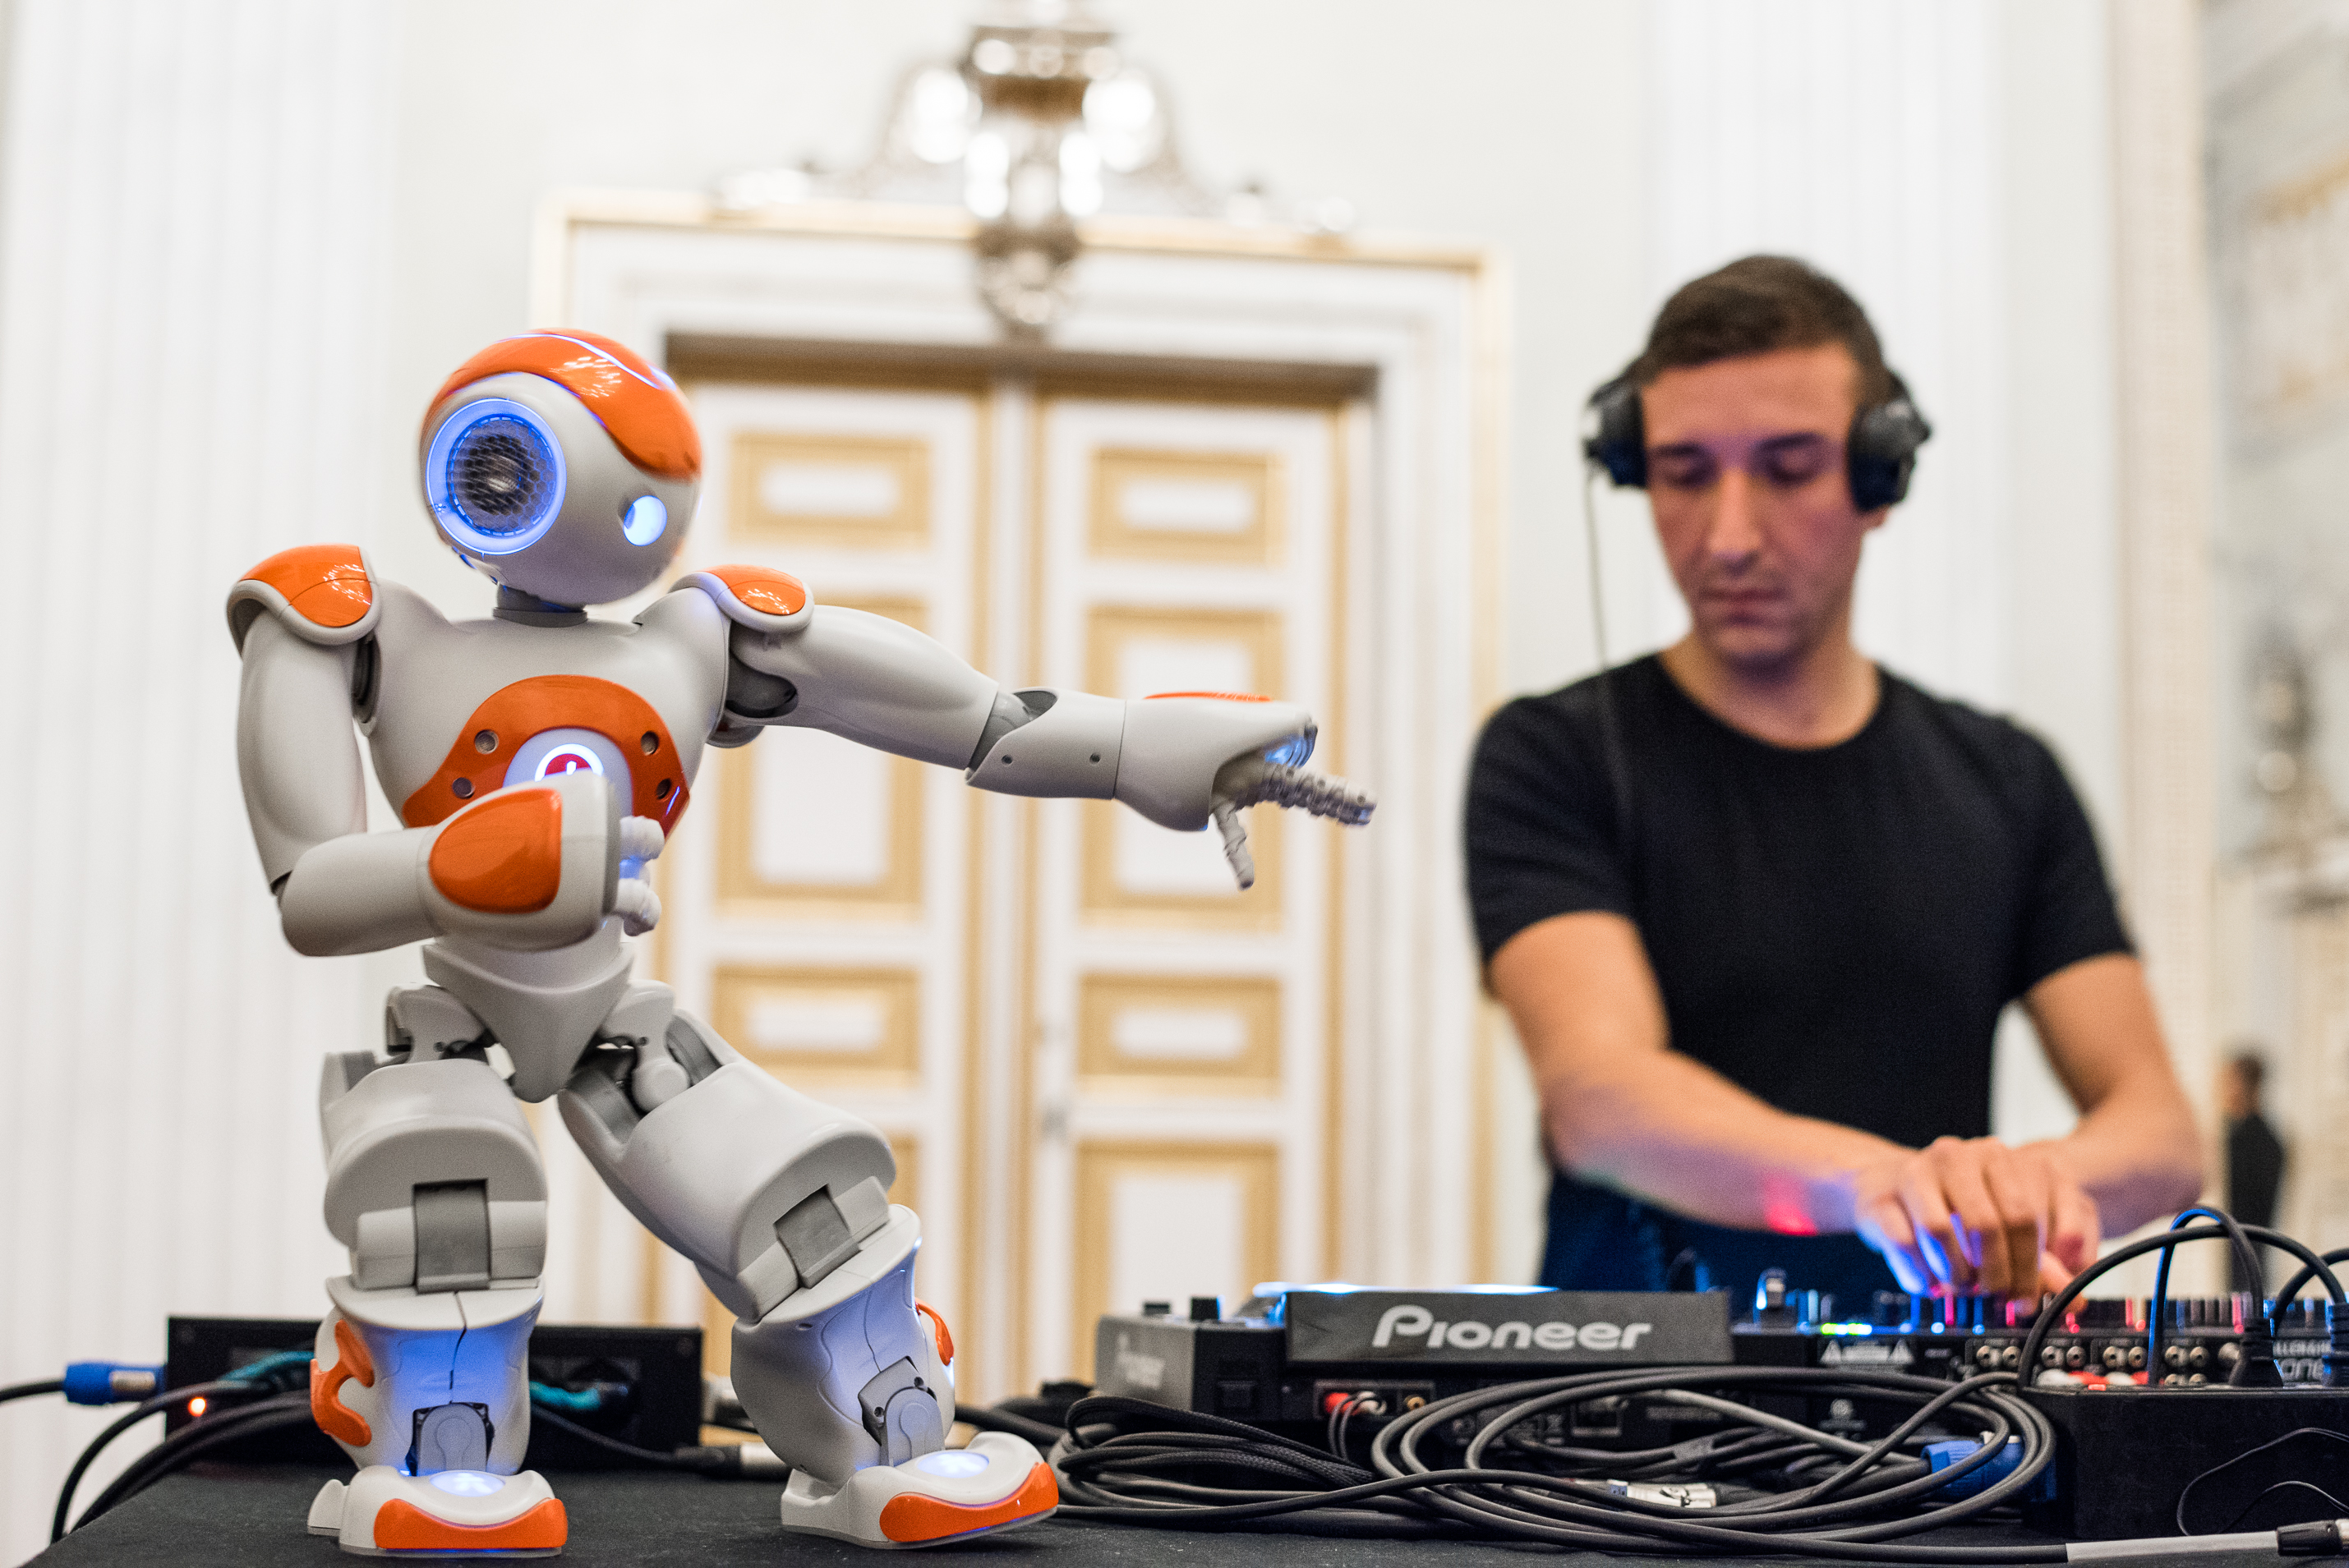
\includegraphics[width=0.9\textwidth]{nao7.jpg}<1->
		\end{center}
		\end{figure}
\end{columns}
\end{frame}

\ifx\fulldocument\undefined
\end{document}
\fi
